\documentclass[conference]{IEEEtran}

\usepackage[utf8]{inputenc} % allow utf-8 input
\usepackage[T1]{fontenc}    % use 8-bit T1 fonts
\usepackage{cite}
\usepackage[pdftex]{graphicx}
\usepackage{amsmath}
\usepackage{amsfonts}
\usepackage{amssymb}
\usepackage{mathtools}
\usepackage{nicefrac}
\usepackage{array}
\usepackage{enumitem}
\usepackage{color}
\usepackage{url}
\usepackage[colorlinks=true,allcolors=black,urlcolor=blue]{hyperref}

%\usepackage{caption}
%\usepackage{subcaption}

%\captionsetup[figure]{textfont=footnotesize,labelfont=footnotesize}

\graphicspath{{images/}}
\DeclareGraphicsExtensions{.pdf,.jpeg,.png}
\interdisplaylinepenalty=2500

% Math commands for matrix and vector fonts
\providecommand{\v}{}
\renewcommand{\v}[1]{\underline{#1}}
\providecommand{\vhat}{}
\renewcommand{\vhat}[1]{\underline{\hat{#1}}}
\providecommand{\m}{}
\renewcommand{\m}[1]{{\bf #1}}
\providecommand{\j}{}
\renewcommand{\j}{\jmath}

% Custom math operators
\DeclareMathOperator*{\argmin}{arg\,min}
\DeclarePairedDelimiter\abs{\lvert}{\rvert}
\DeclarePairedDelimiter\norm{\lVert}{\rVert}
\DeclarePairedDelimiter\floor{\lfloor}{\rfloor}

\newcommand{\Phiorho}{\Phi\!\circ\!\rho}

\renewcommand*\ttdefault{lmtt}

% Theorems, lemmas, etc.
\newtheorem{theorem}{Theorem}
\newtheorem{lemma}[theorem]{Lemma}   % Shares numbering with theorem
\newtheorem{definition}{Definition}

% correct bad hyphenation here
%\hyphenation{op-tical net-works semi-conduc-tor}

\title{Lower Bounds on the Minimax Risk for the \\ Source Localization Problem}

\author{
	\IEEEauthorblockN{
		Praveen Venkatesh (\href{mailto:vpraveen@cmu.edu}{\texttt{vpraveen@cmu.edu}}) %\IEEEauthorrefmark{1}
		and Pulkit Grover (\href{mailto:pulkit@cmu.edu}{\texttt{pulkit@cmu.edu}}) %\IEEEauthorrefmark{2}
	}
	%\IEEEauthorblockA{
	%    Electrical \& Computer Engineering,
	%    and the Center for the Neural Basis of Cognition,
	%    Carnegie Mellon University
	%    \\
	%    \IEEEauthorrefmark{1}\href{mailto:vpraveen@cmu.edu}{\texttt{vpraveen@cmu.edu}}
	%    \IEEEauthorrefmark{2}\href{mailto:pulkit@cmu.edu}{\texttt{pulkit@cmu.edu}}
	%}
}

\begin{document}

\maketitle
\thispagestyle{plain}
\pagestyle{plain}

\begin{abstract}

To be considered for the 2017 IEEE Jack Keil Wolf ISIT Student Paper Award.
The ``source localization'' problem is one in which we estimate the location of
a point source observed through a diffusive medium using an array of sensors.

We give lower bounds on the minimax risk (mean squared-error in location) in
estimating the location of the source, which apply to all estimators, for
certain classes of diffusive media represented by low-pass
filters, when using a uniformly distributed sensor array. We show that
for sensors of a fixed size, the lower bound decays with
increasing numbers of sensors. We also perform a preliminary numerical analysis
to understand the effect of increasing the number of sensors to infinity by
shrinking their size, wherein the bound saturates for large sensor numbers.
In the second scenario, it is seen that there is greater
benefit to increasing the number of sensors as the signal-to-noise increases.
Our bounds are the first to give a scaling for the minimax risk in terms of the
number of sensors used.

%While our results are derived for sources located on a one-dimensional circular
%domain, they can be easily extended to sources on one-dimensional line segments
%and d-dimensional boxes. The technique for deriving these minimax bounds also
%sheds light on the sensor placement problem: increased resolution in a narrow
%region can be obtained by placing sensors \emph{around} the region of interest.

\end{abstract}

\section{Introduction}

The source localization problem arises in many fields in different forms. Our
principal motivation comes from Electroencephalography (EEG), a non-invasive
brain measurement modality which uses electrodes placed on the scalp to sense
electric potentials produced by neuronal activity within the
brain~\cite{Nunez2006Electric}. The neurons (or groups of neurons) which
produce this activity are usually modeled as current dipoles, and it is often
of clinical or neuroscientific interest to estimate their
locations~\cite{Baillet2001Electromagnetic}. For a single activated dipole
within the brain (which is modeled as a point source), the electrodes
effectively sample a diffuse (blurred) representation of the dipole, as a
result of the spatial low-pass filtering effect of the different layers between
the brain surface and scalp surface (cerebrospinal fluid, skull and skin).

Recent developments~\cite{Grover2016Information} have suggested that source
localization can benefit greatly from an increase in sensor density. This
conclusion is based primarily on a Nyquist rate analysis, and on an
information-theoretic bound~\cite{Grover2016Fundamental} on the accuracy of
source localization algorithms. This information-theoretic bound, however, was
derived for the unsampled, continuous-space potential on the scalp, or
equivalently, in the limit of the number of sensors going to infinity. The
claim that source localization can benefit from increased sensor density is,
therefore, not fully substantiated by the information-theoretic bound, since
the latter does not provide a lower bound showing improvement with increasing
sensor density.

Earlier work by Mosher et al.~\cite{Mosher1993Error} also gave numerical lower
bounds on source localization error. However, the Cramer-Rao lower bounds
derived by them do not apply to biased estimators, including several commonly
used source localization
algorithms~\cite{Hamalainen1994Interpreting,Lin2006Assessing}.

This paper seeks to address the shortcomings of earlier methods by deriving
lower bounds on the minimax risk for the source localization problem, which
apply to \emph{all} estimators (biased \emph{and} unbiased), and which captures
how the bound scales with increasing numbers of sensors. Previous lower bounds
are based on ``spherical head
models''~\cite{Nunez2006Electric,Grover2016Information}, which admit analytical
solutions for the potential of a single dipole. But spherical models are not
easily amenable to analytical lower bounds which seek to capture scaling in the
number of sensors, because the spherical surface does not permit uniform
sampling~\cite{Heath1956Thirteen}. We therefore restrict our analysis to a
source localization problem on a one-dimensional ``circular'' domain (to be
described in detail in Section~\ref{sec:source-localization}).

The one-dimensional toy problem is an effective tool for understanding bounds
on source localization accuracy in other settings as well. A vast literature on
linear inverse problems and deconvolution algorithms exists
(see~\cite{Bal2012Introduction} for an introduction to this field), and has
addressed the reduced one-dimensional problem in broad settings
(see~\cite{Cavalier2002Sharp,Efromovich1997Robust,Ibragimov1981Statistical} and
references therein). However, our setting and interpretation appears to be
unique, since most prior work focuses on recovering a whole function (given
certain smoothness constraints), rather than locating a point
source~\cite{Cavalier2002Sharp}. Work that \emph{does} address point sources
and location-based error metrics~\cite{Ibragimov1981Statistical} does not, to
our knowledge, address scaling in the number of sensors.

Hence, we believe that this paper is the first to give lower bounds on source
localization error (measured in an $\ell_2$-distance sense) in estimating the
location of a one-dimensional point source, which is observed by sensors
through a diffusive medium (treated as a low-pass filter), and corrupted by
additive white Gaussian noise. We describe the problem setting in detail in
Section~\ref{sec:source-localization} and the minimax techniques and our main
results (for a naive and then for a more physical sensor model) in
Section~\ref{sec:minimax-lower-bounds}. We conclude in
Section~\ref{sec:discussion} with a discussion on the goodness of our bounds,
and on how our results can be extended to other simple settings.

For EEG source localization, we hope to find algorithms that achieve scalings
close to the bounds we present.  We also expect to build upon the techniques
presented in this paper to derive bounds for spherical and realistic brain
models.

\section{The source localization problem}
\label{sec:source-localization}

We start by giving a detailed description of the one-dimensional setting of the
source localization problem.

\subsection{Description of the domain}

We assume that the point source is located on a circle of circumference $S$. We
use the variable `$s$' to represent a general point on this domain. We can also
view this domain as a line, on which signals are periodic with period $S$.  The
point source is therefore located somewhere within one period. We denote the
set of possible locations by $\Theta = [0, S)$. Due to the periodic nature of
the domain, a source located at position $\theta \in \Theta$ implies the
presence of sources at $s = \theta + kS$,~$\forall \, k \in \mathbb Z$.

\subsection{Sensor configuration}

Sensors are assumed to be uniformly distributed over the domain, i.e., if there
are $m$ sensors, they are placed at locations $s = 0$, $S/m$, $2S/m$,~\dots,
$(m{-}1)S/m$ (the offset of the first sensor is arbitrary, so without loss of
generality we take it to be 0). The periodicity of the space ensures that we
automatically also have sensors at $S$, $S{+}S/m$,~\dots\@ The lower bounds we
provide are for \emph{this specific sensor configuration}. For a discussion on
why this configuration might be an appropriate choice in the minimax setting,
see section~\ref{sec:discussion}.

\subsection{Signal model}
\label{sec:signal-model}

%All ``continuous-space'' signals (analogous to continuous- and
	%discrete-\emph{time} signals) on the aforementioned circular domain are
All signals of the form $f:\Theta\mapsto\mathbb{R}$.  The point source located at $\theta$
is represented by the impulse signal, $f(s;\theta) = \delta(s - \theta)$, where
$\delta(\cdot)$ is the Dirac delta function.  The sensors observe this signal
through the diffusive medium, which, intuitively speaking, blurs the impulse.
More concretely, we assume that the medium is linear and shift-invariant, so
that it can be represented by a spatial impulse response. Then, blurring would
correspond to low-pass filtering.  Let this impulse response be given by
$g(s)$. Then, the noiseless, continuous-space signal (post-filtering and
pre-sampling) is given by the convolution, $x(s; \theta) = (g*f)(s) = g(s -
\theta)$. Here, we further make the simplifying assumption that $g(s)$ has a
sufficiently restricted support, so that aliasing effects are avoided, and
$x(s; \theta)$ is always well-defined. To be precise, $g(s) = 0$ when $\abs{s}
> w/2$, where the ``width'' $w$ of the impulse response satisfies $w < S / 2$
(the reason for the factor of $1/2$ will become clear in a later section). For
the proof, $g(s)$ is also assumed to be Lipschitz continuous with parameter
$\kappa$, i.e., $\abs{g(u) - g(v)} \leq \kappa \abs{u - v} \; \forall \;\; u, v
\in \Theta$.

The sensors sample the shifted continuous-space impulse response, with some
additive noise. We denote the noiseless sampled version of $x(s; \theta)$ by
the $m$-length vector $\v x(\theta)$:
\begin{equation} \label{eq:sampled-signal}
	\v x(\theta) = \bigg[x(0; \theta), \ldots, x\Big(\frac{kS}{m}; \theta\Big), \ldots, x\Big(\frac{(m-1)S}{m}; \theta\Big)\bigg]^T
\end{equation}
where $m$ is the number of sensors and $k \in \{0, 1, \ldots, m-1\}$. The
additive noise is given by $\v \epsilon$ (to be described shortly), and the
noisy samples are represented by
\begin{equation} \label{eq:sensor-obs}
	\v y = \v x(\theta) + \v \epsilon.
\end{equation}
In the source localization problem, we receive $n$ trials\footnote{The word
``trials'' comes from neuroscience literature, where several trials of an
experiment are run with a single participant. The participant is given the same
stimulus in each trial, evoking the same response in the brain (usually with
some trial-to-trial variability). For our purposes, we assume that trials are
effectively i.i.d.\ realizations of sensor noise, with no trial-to-trial
variability.} (i.e., $n$ realizations) of $\v y$ according to
equation~\eqref{eq:sensor-obs}, for the same point source $\theta$, using which
we need to estimate the location of the source.
The complete signal model described in this section is summarized in
Fig.~\ref{fig:signal-model}.

\subsection{Channel model}
\label{sec:channel-model}

The noise $\v \epsilon$, introduced in equation~\eqref{eq:sensor-obs}, is the
only source of uncertainty in the problem. For our purposes, we assume that $\v
\epsilon$ is zero-mean and Gaussian, $\v \epsilon \sim \mathcal{N}(\v 0, \m
\Sigma)$. We restrict our analysis to a ``sensor noise'' setting, wherein
$\m\Sigma = \sigma^2 \m I$, i.e., noise is i.i.d.\ across sensors.

The noise is also assumed to be i.i.d.\ across trials, i.e., the $n$
realizations of $\v y$ are independently drawn from $P(\theta)$, for the
same location parameter $\theta$.

With the addition of Gaussian noise, each possible source location $\theta$
gives rise to a different distribution at the sensors, denoted by $P(\theta) =
\mathcal{N}(\v x(\theta), \m \Sigma)$. $\v y$ is therefore one sample from the
distribution $P(\theta)$. The space of distributions produced by all possible
source locations is $\mathcal{P} = \{P(\theta) : \theta \in \Theta \}$.

\begin{figure}[tp] %  figure placement: here, top, bottom, or page
	\centering
	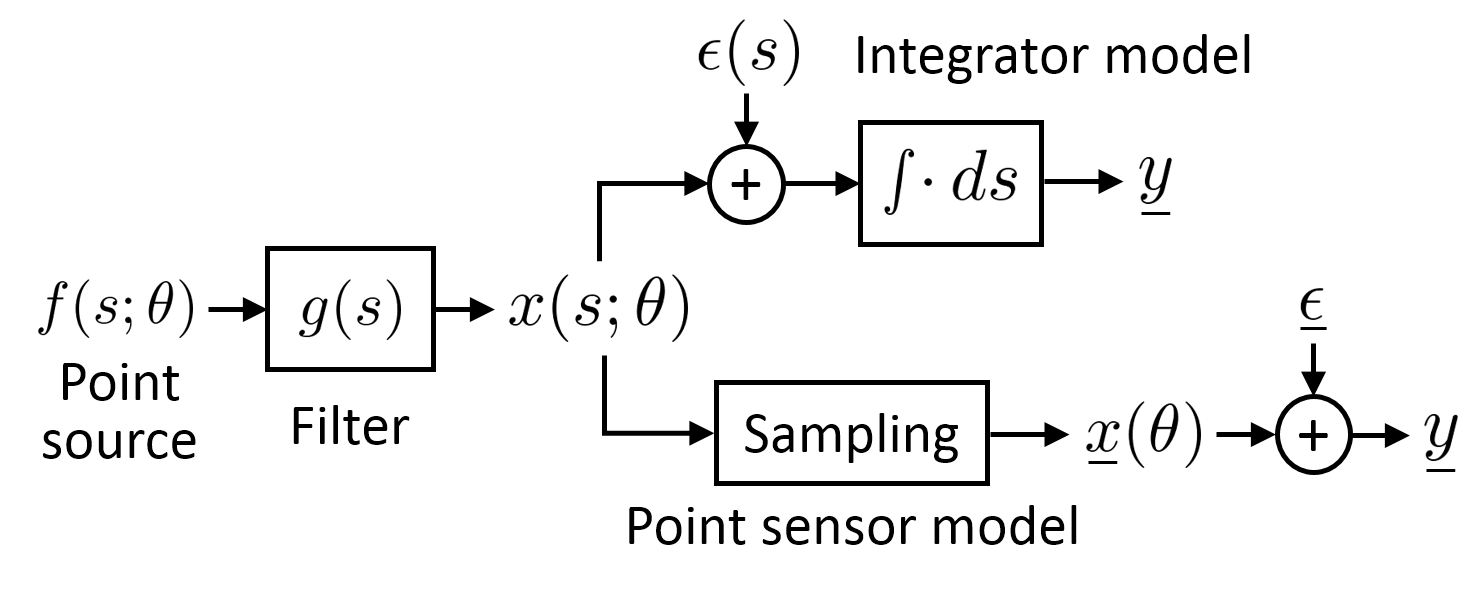
\includegraphics[width=3.5in]{block-diagram}
	\caption{A diagrammatic representation of the signal model described in
	section~\ref{sec:signal-model}.}
	\label{fig:signal-model}
\end{figure}

\section{Lower bounds on the minimax risk for the one-dimensional model}
\label{sec:minimax-lower-bounds}

\subsection{Preliminaries}

Several techniques for deriving lower bounds on the minimax risk are described
in~\cite{Tsybakov2009Introduction}. We follow the excellent tutorial of John
Duchi~\cite{Duchi2015Information} to outline the steps involved.

Consider the following estimation problem: we have $n$ i.i.d.\ random samples
$Y^n$ from a distribution $P$, which is indexed by a parameter $\theta \in
\Theta$.  Denote the set of these distributions by $\mathcal{P} = \{P(\theta) :
\theta \in \Theta\}$. Suppose we now wish to estimate $\theta$ from $Y^n$.
Define a loss metric $\rho(\theta, \hat\theta)$ (e.g.\ $\rho(\theta,
\hat\theta) = \abs{\theta - \hat\theta}$). For this metric, we can define the
minimax risk over all possible estimators $\hat\theta(Y^n)$ and all parameters
$\theta \in \Theta$:
\begin{equation} \label{eq:minimax-expr}
	\mathfrak{M}_n(\mathcal{P}, \Phiorho) = \inf_{\hat\theta} \sup_{\theta \in \Theta} \mathbb E[\Phiorho (\hat\theta(Y^n), \theta)]
\end{equation}
where $\Phi$ is any non-decreasing function (e.g.\ $\Phi(\rho) = \rho^2$).

We start by lower bounding the maximum risk of the estimation problem with the
average risk of a multiple hypothesis testing problem. For this, we first need
to define a $2\delta$-packing.%
\begin{definition}
	A set $\Theta_{\mathcal{V}} = \{ \theta_v : v \in \mathcal{V} \}$ for some
	finite index set $\mathcal{V} \subset \mathbb N$ is said to be a
	$2\delta$-packing in the $\rho$-metric if
	\begin{equation}
		\rho(\theta_i, \theta_j) \geq 2\delta \qquad \forall \;\; \theta_i, \theta_j \in \Theta_{\mathcal{V}}.
	\end{equation}
\end{definition}
\begin{theorem} \label{thm:est-to-testing}%
	If we can find a $2\delta$-packing $\Theta_{\mathcal{V}}$ of $\Theta$, then
	we can lower bound the minimax estimation risk by the average testing risk:
	\begin{equation}
		\mathfrak{M}_n(\mathcal{P}, \Phiorho) \geq \Phi(\delta) \inf_\psi \mathbb P (\psi(Y^n) \neq V)
	\end{equation}
	where $V$ is the unknown true hypothesis which takes values uniformly from
	$\mathcal{V}$, and $\psi$ is our estimate of the hypothesis.
\end{theorem}
For a proof of this theorem, we refer the reader to Proposition~13.3
in~\cite{Duchi2015Information}. Intuitively, Theorem~\ref{thm:est-to-testing}
says that the error in estimating $\theta_i$ is likely to be large if it is
difficult to distinguish $\theta_i$ from $\theta_j$, i.e.\ if the probability
of error is high.

We now need to lower bound the probability of error in the hypothesis testing
problem. The simplest way to do this is to consider a binary hypothesis test
and use what is known as Le Cam's method:
\begin{theorem} \label{thm:le-cam}
	For a binary hypothesis test, i.e., $\mathcal{V} = \{0, 1\}$,
	\begin{equation}
		\inf_\psi \mathbb P(\psi(Y^n) \neq V) = 1 - \norm{P_0 - P_1}_{TV}
	\end{equation}
	where $P_i$ is short-hand for $P(\theta_i)$ and $\norm{P_0 - P_1}_{TV}$ is
	the total variation distance between the two distributions, defined as
	$\norm{\cdot}_{TV} = \frac{1}{2} \norm{\cdot}_1$.
\end{theorem}
For a proof, we refer the reader to Proposition~2.11
in~\cite{Duchi2015Information}. Intuitively, Theorem~\ref{thm:le-cam} states
that the minimum achievable error probability in a binary hypothesis testing
problem is related to the distance between the distributions corresponding to
the two hypotheses.

Thus, the final lower bound can be written as:
\begin{equation} \label{eq:le-cam-bound}
	\mathfrak{M}_n(\mathcal P, \Phiorho) \geq \frac{\Phi(\delta)}{2} \big(1 - \norm{P_1^n - P_0^n}_{TV}\big)
\end{equation}
The superscripts ``$n$'' remind us that these are $n$-fold product
distributions, since we have $n$ i.i.d.\ trials used in the estimate.  The
difficulty in Le Cam's method lies in selecting the two hypotheses to trade-off
the effect due to a small value of $\delta$ and a large value of $\norm{P_1^n -
P_0^n}_{TV}$ appropriately, to derive the tightest possible bound.

\subsection{Lower bounds using Le Cam's method}
\label{sec:lecam-lb}

For the source localization problem, we measure \emph{risk} in terms of the
squared-distance between the true location and the estimated location. Hence,
our loss function is $\Phi(\rho(\theta, \hat\theta)) = \abs{\theta -
\hat\theta}^2$, where $\hat\theta$ is some estimate of the location based on
$n$ trials of the noisy sensor observations $\v y$.

\begin{figure}[t]
	\centering
	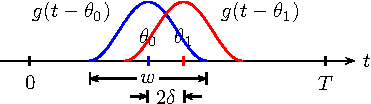
\includegraphics[width=2.6in]{overlap-middle-pics}
	\caption{Depiction of the continuous-space signals produced by two
		hypotheses, $\theta_0$ and $\theta_1$. Note that each signal is a
		shifted impulse response, and therefore has a support of size $w$.
		The set $\{\theta_0, \theta_1\}$ is a $2\delta$-packing of
		$\Theta$, so the signals are separated by a distance $2\delta$.}
	\label{fig:overlap-middle}
\end{figure}
\begin{figure}[t]
	\centering
	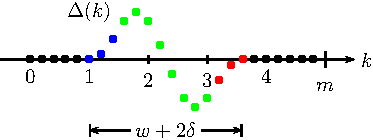
\includegraphics[width=2.6in]{delta-sampled-pics}
	\caption{Plot of the samples of the difference signal, $\Delta(k)$. The
		total size of the support of the difference signal is $w+2\delta$,
		hence at most $\floor*{\frac{(w + 2\delta)m}{S} + 1}$ samples of
		$\Delta(k)$ are non-zero.}
	\label{fig:delta-sampled}
\end{figure}

We now state the main result of this paper.
\begin{theorem} \label{thm:main-lb}
	For a source localization problem as defined in
	section~\ref{sec:source-localization}, the minimax risk in estimating the
	location of a point source is lower bounded by
	\begin{equation}
		\mathfrak{M}_n(\mathcal{P}, \Phi\circ\rho) \geq \sup_{0 < \delta < S/4} \frac{\delta^2}{2} \Bigg[1 - \sqrt{\frac{2n \kappa^2 \delta^2}{\sigma^2}\bigg(\!\frac{(w{+}2\delta) m}{S} + 1\!\bigg)} \Bigg]
	\end{equation}
	For sufficiently large $m$, the bound can be approximated by
	\begin{equation} \label{eq:main-lower-bound}
		\mathfrak{M}_n(\mathcal{P}, \Phiorho) \gtrsim \frac{1}{32} \frac{\sigma^2 S}{nm\kappa^2w}.
	\end{equation}
\end{theorem}%
\begin{IEEEproof}
Starting from equation~\eqref{eq:le-cam-bound}, we proceed to derive the total
variation distance for the distributions of interest. Using Pinsker's
inequality~\cite{Kullback1967Lower} and the convenient tensorization of the
KL-divergence~\cite{Duchi2015Information}, we see that:
\begin{equation} \label{eq:pinsker-tensorization}
	\norm{P_1^n - P_0^n}_{TV}^2 \leq \frac{1}{2} D_{KL}(P_0^n \Vert P_1^n) = \frac{n}{2} D_{KL}(P_0 \Vert P_1)
\end{equation}
For multivariate normal distributions with the same covariance, the
KL-divergence is given by
\begin{equation} \label{eq:kl-div-normal}
	D_{KL}(P_0 \Vert P_1) = (\v \mu_0 - \v \mu_1)^T \m \Sigma^{-1} (\v \mu_0 - \v \mu_1)
\end{equation}
where $\v \mu_0$ and $\v \mu_1$ are the means of $P_0$ and $P_1$
respectively~\cite{DuchiDerivation}. For the case of sensor noise, $P_i =
\mathcal{N}(\v x(\theta_i), \sigma^2 \m I)$, as described in
section~\ref{sec:channel-model}. Hence, combining
equations~\eqref{eq:le-cam-bound}, \eqref{eq:pinsker-tensorization} and
\eqref{eq:kl-div-normal}, we see that
\begin{equation} \label{eq:lb-after-pinsker}
	\mathfrak{M}_n(\mathcal{P}, \Phiorho) \geq \frac{\delta^2}{2} \Bigg[ 1 - \sqrt{ \frac{n}{2\sigma^2} \norm*{\v x(\theta_0) - \v x(\theta_1)}^2 } \Bigg]
\end{equation}
Let $\v \Delta \overset{\text{def.}}{=} \v x(\theta_0) - \v x(\theta_1)$ for
brevity. Also, let $\Delta(k)$ denote the $k$-th element of $\v\Delta$, and
$\mathbb I_A(k)$ denote the indicator function of $k$ belonging to the set $A$
(i.e., $\mathbb I_A(k) = 1$ if $k \in A$, and $0$ otherwise). Then, we have
\begin{align}
	&\norm{\v\Delta}^2 = \sum_{k=0}^{m-1} \abs{\Delta(k)}^2 = \sum_{k=0}^{m-1} \abs{\Delta(k)}^2 \, \mathbb I_{\{\ell: \abs{\Delta(\ell)} \neq 0\}}(k) \\
	&= \sum_{k=0}^{m-1} \abs[\Big]{x\Big(\frac{kS}{m}; \theta_0\Big) - x\Big(\frac{kS}{m}; \theta_1\Big)}^2 \mathbb I_{\{\ell: \abs{\Delta(\ell)} \neq 0\}}(k) \\
	&= \sum_{k=0}^{m-1} \abs[\Big]{g\Big(\frac{kS}{m} - \theta_0\Big) - g\Big(\frac{kS}{m} - \theta_1\Big)}^2 \mathbb I_{\{\ell: \abs{\Delta(\ell)} \neq 0\}}(k)
\end{align}
where $x(s;\theta_i)$ is the continuous-space filtered signal described in
section~\ref{sec:signal-model}. For an impulse response $g$ which is Lipschitz
continuous with parameter $\kappa$, we can upper bound the term within the
summation:
\begin{equation}
	\abs[\Big]{g\Big(\frac{kS}{m} - \theta_0\Big) - g\Big(\frac{kS}{m} - \theta_1\Big)} \leq \kappa \abs{\theta_0 - \theta_1} = \kappa \cdot 2\delta
\end{equation}
since $\abs{\theta_0 - \theta_1} = 2\delta$ by virtue of the $2\delta$ packing.
Hence,
\begin{equation}
	\norm{\v\Delta}^2 \leq 4 \kappa^2 \delta^2 \sum_{k=0}^{m-1} \mathbb I_{\{\ell: \abs{\Delta(\ell)} \neq 0\}}(k) = 4 \kappa^2 \delta^2 \norm{\v\Delta}_0.
\end{equation}
$\norm{\v\Delta}_0$ is the number of non-zero elements in $\v\Delta$, which is
equal to the number of sensors in the total region covered by the signals
$x(s;\theta_0)$ and $x(s;\theta_1)$ (see Figs.~\ref{fig:overlap-middle} and
\ref{fig:delta-sampled}). Therefore, $\norm{\v\Delta}_0 = \floor[\big]{\frac{(w
+ 2\delta)m}{S} + 1}$, since at most a fraction $(w + 2\delta) / S$ of the $m$
sensors (plus 1, to account for edge-effects) can lie in the region covered by
the two impulse responses. The final upper bound on $\norm{\v\Delta}^2$ is
hence
\begin{equation} \label{eq:delta-bound}
	\norm{\v\Delta}^2 \leq 4 \kappa^2 \delta^2 \floor*{\frac{(w + 2\delta)m}{S} + 1} \leq 4 \kappa^2 \delta^2 \Big(\frac{(w + 2\delta) m}{S} + 1\Big).
\end{equation}
Since sensors are uniformly distributed, and since the domain is periodic, this
holds even if $\theta_0$ lies at the edge of the domain (close to $s=0$, for
example). In such a case, one part of the signal $x(s;\theta_0)$ will appear at
the left edge of the domain, and the remaining part will appear as the
repetition from the period $[S, 2S)$, at the right edge of the domain. Also
note that the two signals $x(s;\theta_0)$ and $x(s;\theta_1)$ overlap at most
once, since $w < S/2$, as stated in section~\ref{sec:signal-model}.

Combining equations~\eqref{eq:lb-after-pinsker} and~\eqref{eq:delta-bound},
\begin{equation} \label{eq:lb-after-delta-bound}
	\mathfrak{M}_n(\mathcal{P}, \Phiorho) \geq \frac{\delta^2}{2} \Bigg[1 - \sqrt{\frac{2n \kappa^2 \delta^2}{\sigma^2}\bigg(\!\frac{(w{+}2\delta) m}{S} + 1\!\bigg)} \Bigg].
\end{equation}
This bound holds for any feasible $2\delta$-packing. We can derive the tightest
possible bound by maximizing the above quantity over all feasible $\delta$.
Since the maximum attainable separation between two hypotheses on the periodic
domain is $S/2$, we maximize $\delta$ over $(0, S/4)$. This yields the theorem.

To derive the approximation, we observe that for sufficiently large numbers of
sensors, the optimal value of $\delta$ starts becoming small, as hypotheses
must chosen to be closer in order to make the error probability large. Hence,
neglecting edge effects and terms of order $\delta^3$, we can give an
approximate bound for large $m$ using a heuristic: tighten the bound by
choosing $\sqrt{\frac{2n\kappa^2\delta^2wm}{\sigma^2 S}} = \frac{1}{2}$. This
is achieved for $\delta = \sqrt{\frac{\sigma^2 S}{8nm\kappa^2 w}}$, so that for
$\Phi(\delta) = \delta^2$, equation~\eqref{eq:lb-after-delta-bound} becomes
\begin{equation}
	\mathfrak{M}_n(\mathcal{P}, \Phiorho) \gtrsim \frac{1}{32} \frac{\sigma^2 S}{nm\kappa^2 w}.
\end{equation}
This completes the proof.
\end{IEEEproof}

\subsection{Towards a more physical sensor model}

The bound in Theorem~\ref{thm:main-lb} may mislead one to think that the error
in source localization goes to zero, as the number of sensors goes to infinity.
This observation is contradicts the information-theoretic lower bound given
in~\cite{Grover2016Fundamental}, where even with an infinite number of sensors,
the lower bound is strictly greater than zero. This indicates that the bound in
section~\ref{sec:lecam-lb} is failing to capture some effect which leads to
saturation of error as the number of sensors increases.

Indeed, the bound in Theorem~\ref{thm:main-lb} assumes that an arbitrarily
large number of sensors can be squeezed into a finite amount of space, and that
these sensors \emph{still} have the same SNR.  This is non-physical, since in
reality, each sensor has a certain width, and the value measured by it is the
integral of the continuous-space signal within that width (analogous to a
sample-and-hold circuit, which integrates a continuous-\emph{time} signal over
a short period).  If the width of a sensor is decreased, then effectively, its
SNR reduces.  This is intuitively evident in the sample-and-hold analogy: to
compute the signal value, the integral must be divided by the time interval
over which the integration is performed; this division amplifies noise as the
time interval gets smaller.

We performed a preliminary study to understand the effect of viewing sensors as
integrators. In the new sensor model, sensors have a width which decreases as
their number grows to infinity. Concretely, the $k$-th sensor which is located
at $s = kS/m$ extends from $(k{-}\frac{1}{2})S/m$ to $(k{+}\frac{1}{2})S/m$.
The signal sensed by this sensor is the $k$-th element of $\v x(\theta)$, now
given by
\begin{equation}
	x_k(\theta) = \int_{(k-\frac{1}{2})S/m}^{(k+\frac{1}{2})S/m} x(s;\theta) ds
\end{equation}
The noise vector $\v \epsilon$ is also generated similarly, by integrating over
small sections of a white noise process, which is assumed to additively corrupt
the continuous-space signal $x(s;\theta)$ prior to sampling. This leads to
i.i.d.\ noise values at sensors (since they do not overlap), with variance
inversely proportional to $m$, i.e., $\sigma(m) \propto 1/\sqrt{m}$.

The bounding technique used in section~\ref{sec:lecam-lb} no longer easily
admits a closed-form solution which gives a bound for all values of $m$. We
instead compute the bound numerically, using exact expressions for error
probability in a binary hypothesis test. For Gaussian distributions of equal
variance and a uniform prior on the hypotheses, the minimum possible error
probability (over all tests) is a $Q$-function in the distance between their
means~\cite{NPLemmaOrSimilar},
\begin{equation}
	P_e = \inf_\psi \mathbb P(\psi(Y^n) \neq V) = Q\bigg(\frac{\norm{\v\mu_0 - \v\mu_1}}{2\sigma(m)}\bigg).
\end{equation}
where $Q(x) = \int_x^\infty \frac{1}{\sqrt{2\pi}} e^{-u^2/2} du$. Hence, from
Theorem~\ref{thm:est-to-testing},
\begin{equation}
	\mathfrak{M}_n(\mathcal{P}, \Phiorho) \geq \Phi(\delta) P_e = \delta^2 Q\bigg(\frac{\norm{\v x(\theta_0) - \v x(\theta_1)}}{2\sigma(m)}\bigg).
\end{equation}
This bound is valid for any $\{\theta_0, \theta_1\}$ constituting a
$2\delta$-packing of $\Theta$. To numerically optimize over all possible
packings, we relax the process by fixing $\theta_0 = 0$ and optimizing over
$\theta_1 = 2\delta$.  We compute sensor values by performing numerical
integration, and find the best possible $\delta$ by grid search.

\begin{figure}[t]
	\centering
	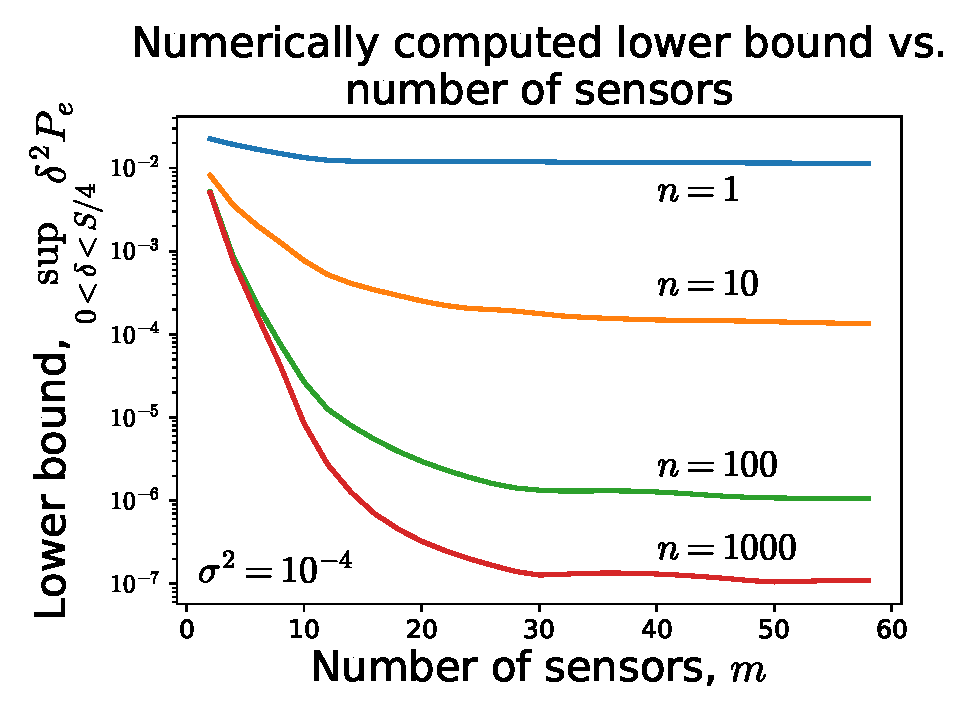
\includegraphics[width=2.8in]{lb-vs-m-annotated}
	\caption{A numerically generated plot of the lower bound on minimax risk of
		source localization, against the number of uniformly distributed
		sensors, $m$, used to estimate the location. The different curves are
		for different numbers of ``trials'' $n$ (i.i.d.\ sensor observations).
		The bound saturates for large $m$, indicating that for a fixed number
		of trials (or equivalently, for a fixed SNR), there is reduced benefit
		in increasing the number of sensors beyond a point. However, with more
		trials, the bound saturates at increasingly larger numbers of sensors.
	Thus, there is benefit to increasing the number of sensors, provided SNR
can be increased by leveraging larger numbers of trials.}
	\label{fig:numerical}
\end{figure}

Plotting this numerically computed bound for different numbers of trials (see
Fig.~\ref{fig:numerical}) reveals some interesting trends. First, the bound
saturates as $m$ grows large, matching the behaviour presented
in~\cite{Grover2016Fundamental}. Second, the lower bound on error is larger for
smaller numbers of sensors, as we expect. Third and most importantly, as the
number of trials increases, bound begins to saturate only for larger numbers of
sensors. In other words, there is increased benefit in using larger numbers of
sensors, when we also have more trials\footnote{Recall that the number of
``trials'' is the number of i.i.d.\ sensor observations we receive, per
equation~\ref{eq:sensor-obs}.}. This substantiates the intuition given
in~\cite{Grover2016Information}, which addresses this issue using a
Nyquist-rate perspective. A larger number of sensors will sample a larger
number of high-frequency components of the source signal (and hence allow us to
locate it better), but only if the noise floor is sufficiently low. Noise
variance, in turn, can be reduced by averaging over multiple trials.

\section{Discussion}
\label{sec:discussion}

While the lower bound presented in section~\ref{sec:lecam-lb} is non-physical
for a large number of sensors, it still gives some important insights. For
instance, if we assume that sensors have a constant width $c$, then even if we
view sensors as integrators, the bound tells us something about the scaling of
error with number of sensors, up to $m = \floor*{\frac{S}{c}}$. Beyond this
point, averaging noise by increasing the number of trials may help one get to a
target mean squared error in location. An analytical derivation of the
trade-off between $m$ and $n$ in achieving a certain target MSE is relegated to
future work.

We also note that the minimax bounds from compressive sensing
literature~\cite{AriasCastro2013Fundamental} do not apply in our setting,
because those consider the problem of recovering the whole source signal,
$x(s;\theta)$. The loss function used there is hence the energy of the
difference signal $\int \abs{x(s) - \hat x(s)}^2 ds$. We, on the other hand,
are interested in bounding the minimax error in \emph{location}, i.e.,
$\abs{\theta - \hat\theta}^2$.

While the bounds in section~\ref{sec:lecam-lb} were derived for a
one-dimensional circular domain, extensions to a one-dimensional linear domain
(of fixed length) and to a $d$-dimensional domain (circular or linear) are
fairly straightforward, under certain conditions. For a 1D linear domain, we
require that sensors capture the entirety of the impulse response even at the
edges of the domain. Hence, sensors must be placed uniformly in $[-w/2,
S{+}w/2]$. For extending to $d$ dimensions, it suffices to apply Assouad's
Lemma~\cite{Tsybakov2009Introduction} to separate the problem into $d$
independent one-dimensional problems. Such extensions substantially broaden the
number of settings in which this bound applies.

Another point on sensor placement bears repeating: the bounds derived in this
paper apply to only a specific sensor configuration, i.e., the uniform one.
Intuitively, this is the correct choice in the minimax setting, since any
non-uniform placement will have one or more points which is far from all
sensors. The ``maximization'' over $\theta \in \Theta$ would then select a
$\theta$ for which the value of the impulse response at the sensors is
smallest, so that the ratio of mean-sensor-value to noise variance (a form of
SNR) is minimized.

%The lower bounding \emph{technique} itself gives certain inisights on the issue
%of sensor placement. Suppose we wanted to achieve a higher resolution in a
%restricted interval of the parameter space, i.e.\ $\theta \in [a, b] \subset
%\Theta$, such that $\abs{b - a} \ll w$. Then, it might be of greatest benefit
%to place sensors \emph{not} precisely over $[a, b]$, but rather in the region
%\emph{surrounding} $[a, b]$, corresponding to the \emph{largest change} in the
%impulse response. Indeed, it is possible to derive an approximate lower bound
%using Taylor's approximation, which shows that the KL-divergence between
%distributions is maximized (and hence error minimized) at regions where the
%slope of $x(s;\theta)$ is largest.

%\section{Extensions}
%\label{sec:extensions}

%\subsection{From a circular (periodic) domain to a linear (aperiodic) domain}

%So far, we've relied on the presence of a circular domain for to make the
%arguments in the proof. However, the most important requirement was that
%\emph{all} parts of the impulse response should get \emph{sensed} uniformly.
%So, if $\theta$ were restricted to the region $[0, S)$ (now on a linear,
%non-periodic domain), and if sensors were available to sense the signal from
%$[-w/2, S{+}w/2)$ (for an impulse response with restricted support as described
%in section~\ref{sec:signal-model}), then the proof for sensor noise would still
%fall through, albeit with slightly different constants.

%\subsection{From Lipschitz to $\alpha$-Holder continuous impulse responses}

%We can trivially expand the domain of impulse responses to which the lower
%bound in~\eqref{eq:main-lower-bound} applies to include $\alpha$-Holder
%continuous functions. These are functions which satisfy
%\begin{equation}
%    \abs{g(u) - g(v)} \leq \kappa \abs{u - v}^\alpha \, \forall \, u, v \in \text{dom} \; g
%\end{equation}
%for some constant $\kappa$, and for $\alpha > 0$. Using this property,
%equation~\eqref{eq:delta-bound} reads
%\begin{equation} \label{eq:holder-delta-bound}
%    \norm{\v\Delta}^2 \leq \kappa^2 (2 \delta)^{2\alpha} \bigg(\frac{(w + 2\delta) m}{S} + 1\bigg).
%\end{equation}
%Hence, we choose $\delta = (\frac{\sigma^2 S}{2^{2\alpha + 1} nm \kappa^2
%w})^{1/2\alpha}$, to procure an asymptotic lower bound
%\begin{equation}
%    \mathfrak{M}_n(\mathcal{P}, \Phiorho) \geq \frac{1}{4} \bigg(\frac{\sigma^2 S}{2^{2\alpha + 1} nm \kappa^2
%w}\bigg)^{1/\alpha}.
%\end{equation}

%\subsection{From a one-dimensional domain to a $d$-dimensional domain}

%Another simple extension takes our problem from a one-dimensional setting to a
%$d$-dimensional setting. Here, we would have $\v\theta \in [0, S)^d$, and the
%$\ell_2$ loss function, $\Phiorho(\v\theta, \vhat\theta) = \norm{\v\theta -
%\vhat\theta}^2$. Then, using Assouad's lemma~\cite{Tsybakov2009Introduction} in
%the manner described in~\cite{Duchi2015Information}, we can split the minimax
%risk along each of the $d$ dimensions, and bound each separately using Le Cam's
%method.

%\IEEEtriggeratref{8}

\bibliographystyle{IEEEtran}
\bibliography{IEEEabrv,references}

\end{document}
